\documentclass[aspectratio=169,11pt]{beamer}
\usetheme[progressbar=frametitle,numbering=fraction]{metropolis}
\usepackage[utf8]{inputenc}
\usepackage[T1]{fontenc}
\usepackage[spanish,es-noshorthands]{babel}
\usepackage{booktabs}
\usepackage{amsmath}
\graphicspath{{../informe/figures/}}

\definecolor{verde}{HTML}{1B5E20}
\definecolor{cafe}{HTML}{795548}
\setbeamercolor{frametitle}{bg=verde}
\setbeamercolor{progress bar}{fg=cafe}
\setbeamercolor{alerted text}{fg=cafe}

\title{Deslizamientos cosísmicos del sismo $M_w$~7.4 de San José del Palmar (Chocó)}
\subtitle{Detección de cambios con Sentinel-2: $\Delta$NDVI, $\Delta$NIR y post-clasificación Random Forest}
\author{Jorge Sierra \and Hania Valentina Carreño \and Andrés Felipe Barrios Bohórquez \and Nicolás León Parra}
\date{Proyecto de Medio Semestre -- Entrega final}

\begin{document}

\maketitle

% ---------------------------------------------------------------
\begin{frame}{El evento y el área de estudio}
\begin{columns}[T]
\column{0.5\textwidth}
\begin{itemize}
  \item \textbf{10 de agosto de 2026}, 12:34 UTC, $M_w$~7.4, profundidad $\sim$110 km (SGC).
  \item Desastre nacional; Copernicus EMS activó el \textbf{EMSR916}.
  \item Vías a San José del Palmar bloqueadas por deslizamientos: municipio aislado.
  \item \textbf{ROI:} 49.7 km$^2$ en el cañón del río Ingará y el casco urbano.
  \item Laderas empinadas con bosque húmedo y pastos: muy susceptibles.
\end{itemize}
\column{0.5\textwidth}
\centering
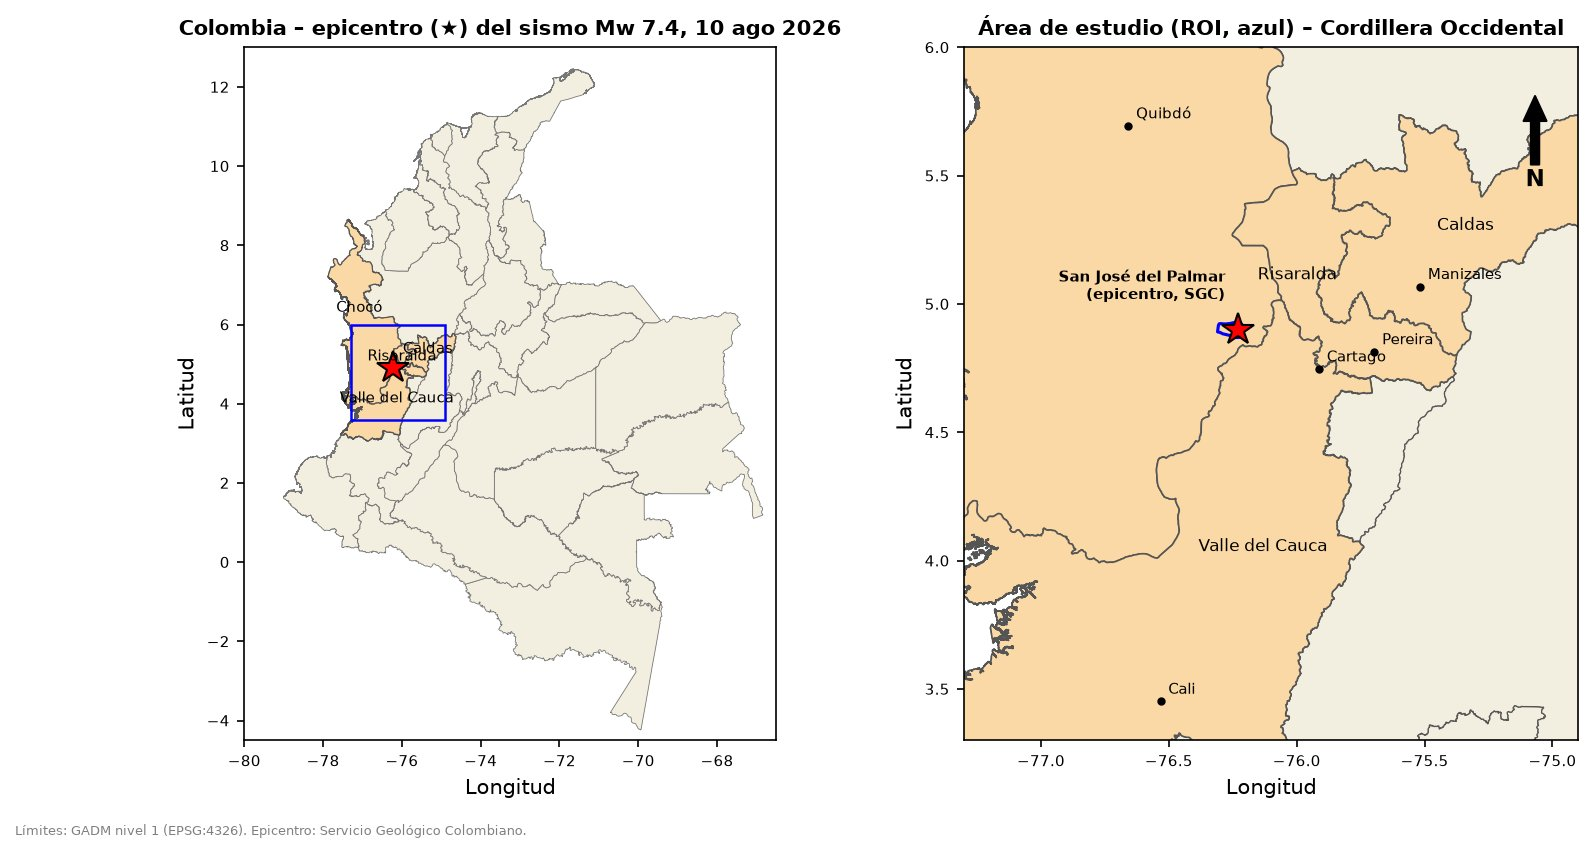
\includegraphics[width=\linewidth,height=0.72\textheight,keepaspectratio]{fig_location.jpg}
\end{columns}
\end{frame}

% ---------------------------------------------------------------
\begin{frame}{Fase 1 -- Datos}
\begin{columns}[T]
\column{0.38\textwidth}
\begin{itemize}
  \item Sentinel-2 MSI \textbf{L2A} (reflectancia BOA), Copernicus Browser.
  \item $t_1$ = \textbf{24-jul-2026} (antes).
  \item $t_2$ = \textbf{18-ago-2026} (después; el 10-ago estaba nublado).
  \item Bandas B02, B03, B04, B08, B11, B12 + SCL, a 10 m.
\end{itemize}
\column{0.31\textwidth}\centering
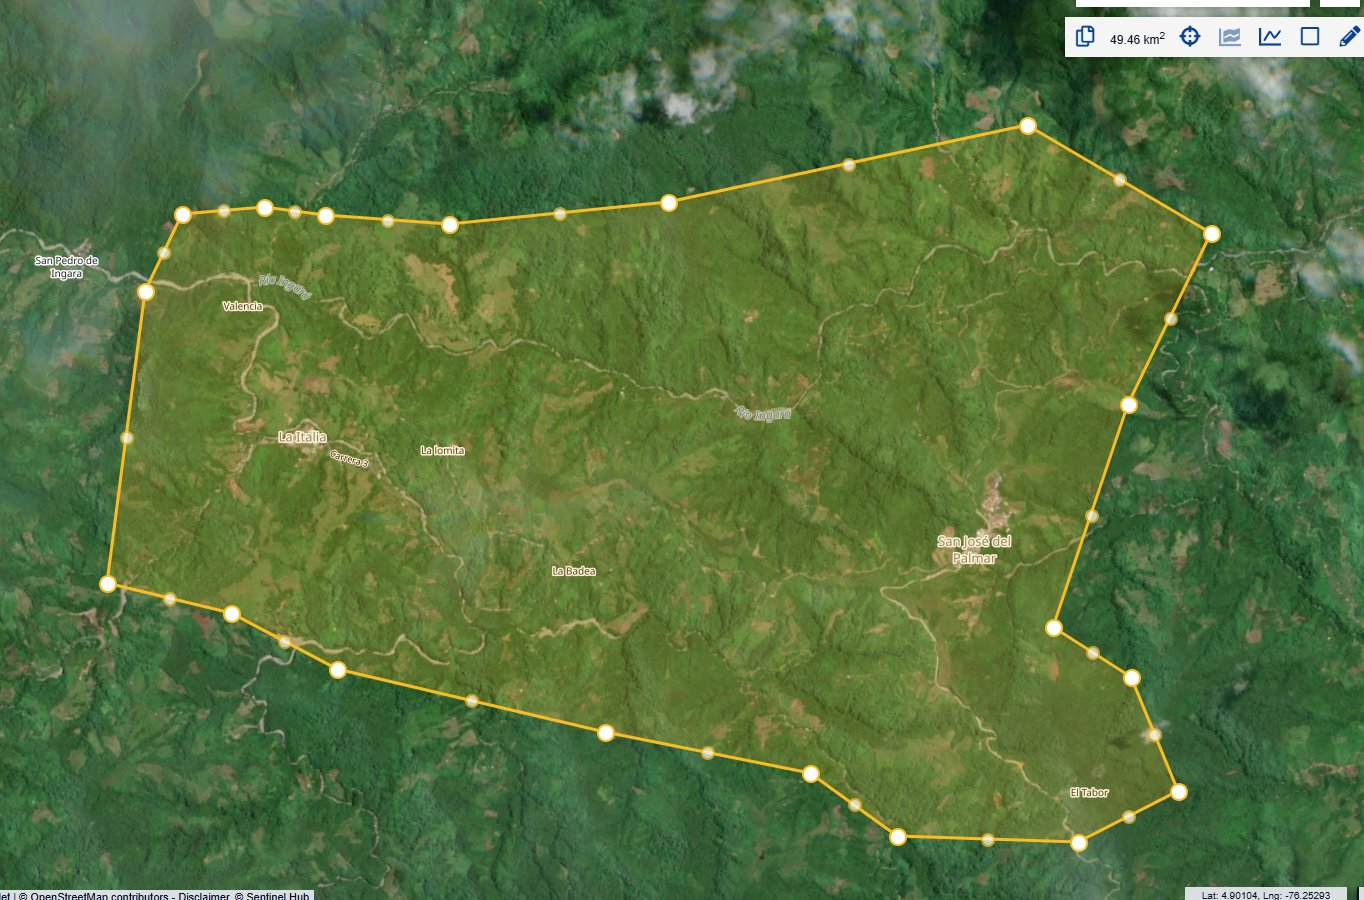
\includegraphics[width=\linewidth]{cap_aoi_t1.jpg}\\[-1mm]{\small $t_1$}
\column{0.31\textwidth}\centering
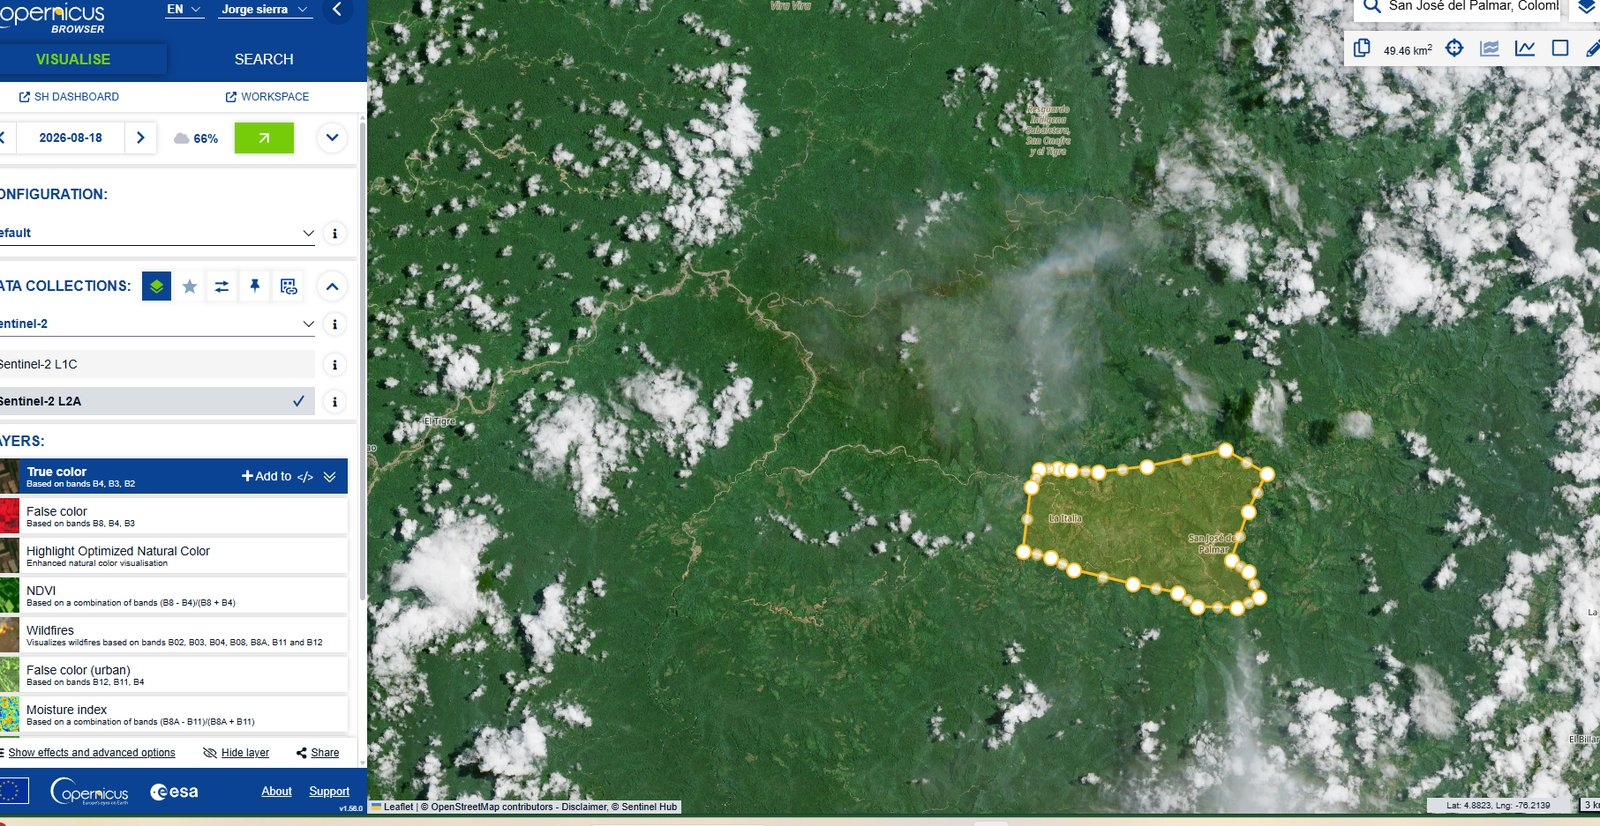
\includegraphics[width=\linewidth]{cap_aoi_t2.jpg}\\[-1mm]{\small $t_2$}
\end{columns}
\end{frame}

% ---------------------------------------------------------------
\begin{frame}{Fase 2 -- Preprocesamiento}
\begin{columns}[T]
\column{0.5\textwidth}
\begin{itemize}
  \item \textbf{Align Rasters}: EPSG:9377, grilla común 10 m (1054 $\times$ 681), referencia \texttt{t1\_B04}.
  \item Bilineal para bandas, vecino más cercano para SCL.
  \item \textbf{Máscara de nubes}: SCL decodificada por color.
  \item En $t_1$, además, $B02 \le 0.1$: nubes que la SCL no detectó.
  \item En $t_2$ la SCL detectó \textbf{cirros} invisibles a simple vista.
  \item Área válida: \textbf{47.2 km$^2$ (94.9\%)}.
\end{itemize}
\column{0.25\textwidth}\centering
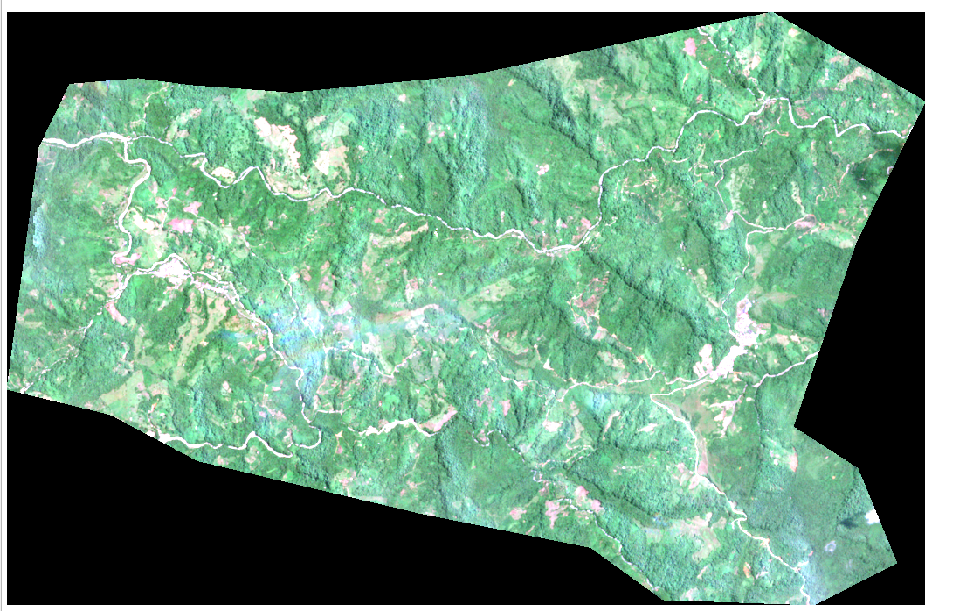
\includegraphics[width=\linewidth]{q_cirro_t2.png}\\{\small cirros en $t_2$}
\column{0.25\textwidth}\centering
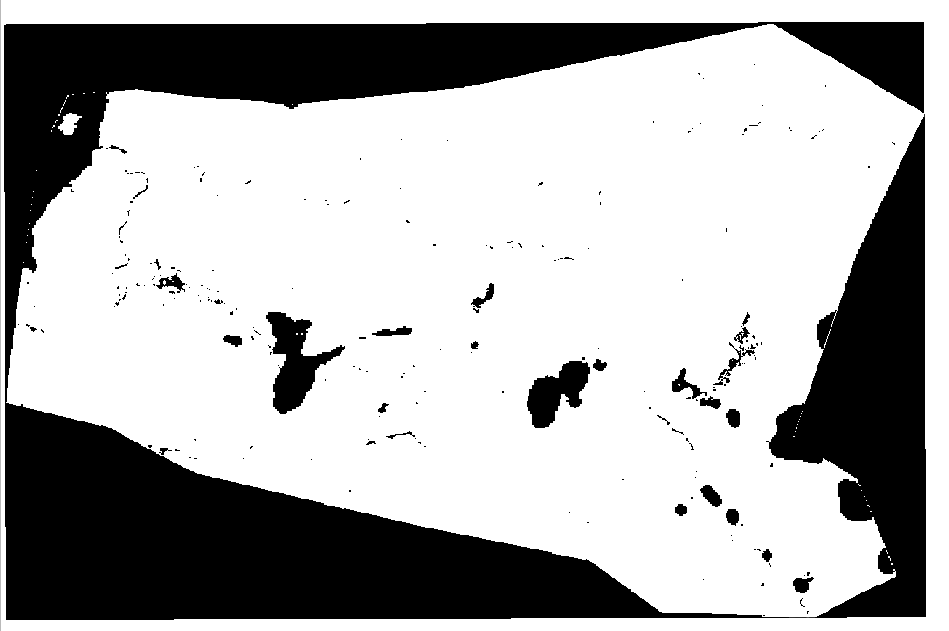
\includegraphics[width=\linewidth]{q_valid.png}\\{\small máscara \texttt{valid}}
\end{columns}
\end{frame}

% ---------------------------------------------------------------
\begin{frame}{Antes y después}
\begin{columns}[T]
\column{0.5\textwidth}\centering
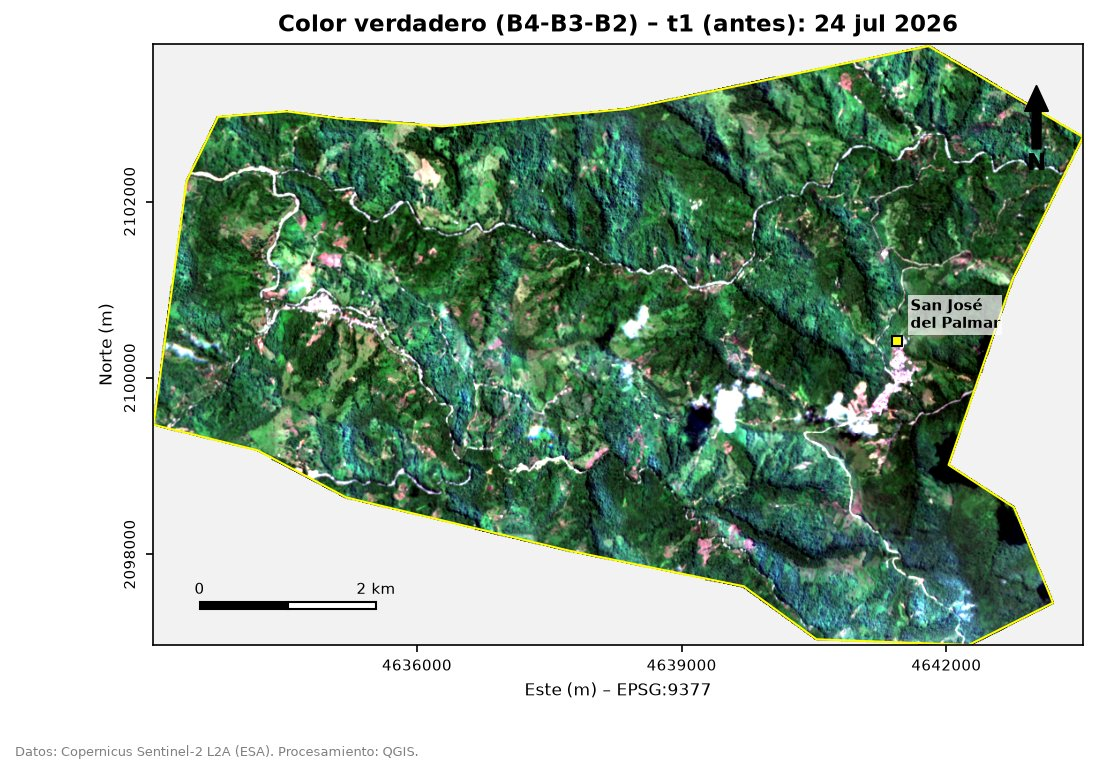
\includegraphics[width=\linewidth,height=0.7\textheight,keepaspectratio]{fig_t1_truecolor.jpg}\\{\small $t_1$ -- 24 de julio}
\column{0.5\textwidth}\centering
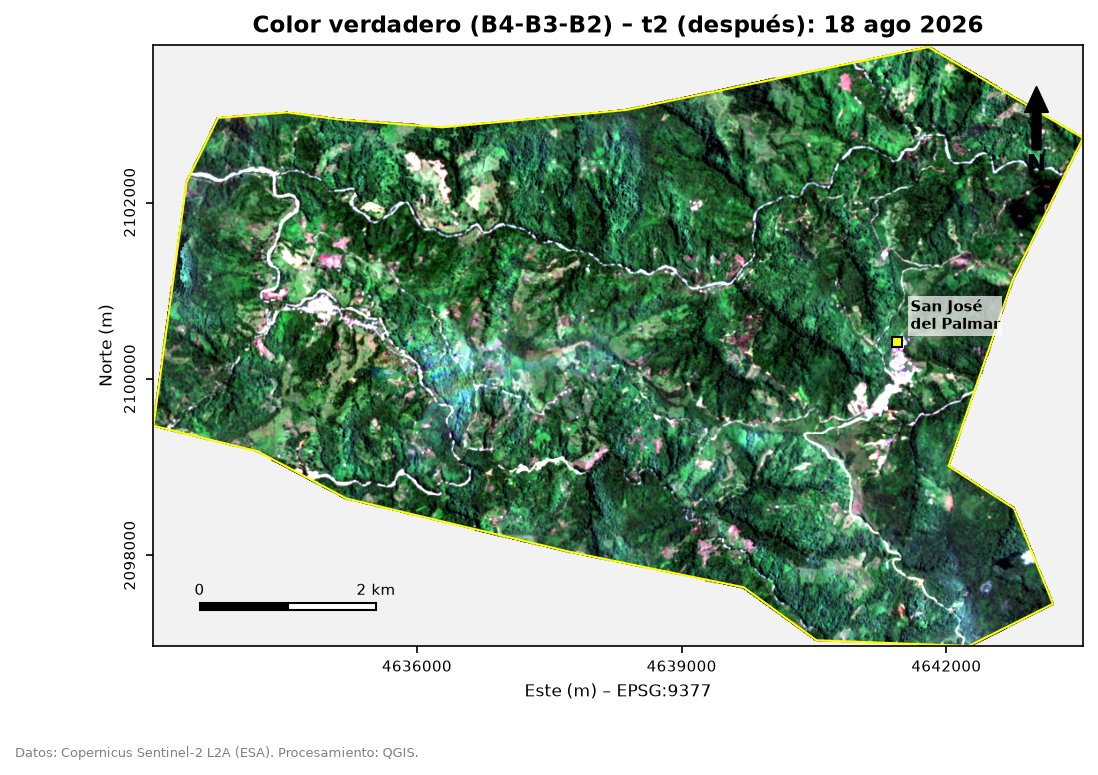
\includegraphics[width=\linewidth,height=0.7\textheight,keepaspectratio]{fig_t2_truecolor.jpg}\\{\small $t_2$ -- 18 de agosto: nuevas cicatrices de suelo}
\end{columns}
\end{frame}

% ---------------------------------------------------------------
\begin{frame}{Fase 3 -- $\Delta$NDVI y $\Delta$NIR}
\begin{columns}[T]
\column{0.5\textwidth}\centering
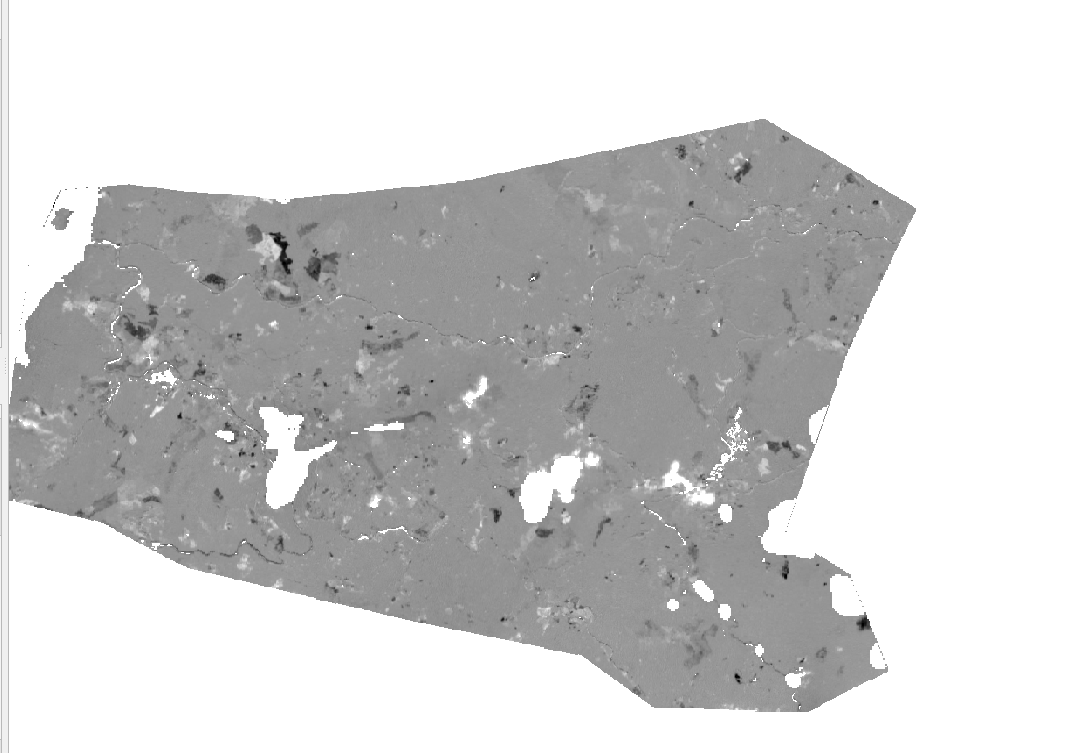
\includegraphics[width=\linewidth,height=0.6\textheight,keepaspectratio]{q_dndvi.png}\\
{\small $\Delta NDVI = NDVI_{t_2} - NDVI_{t_1}$ \quad (oscuro = pérdida)}
\column{0.5\textwidth}\centering
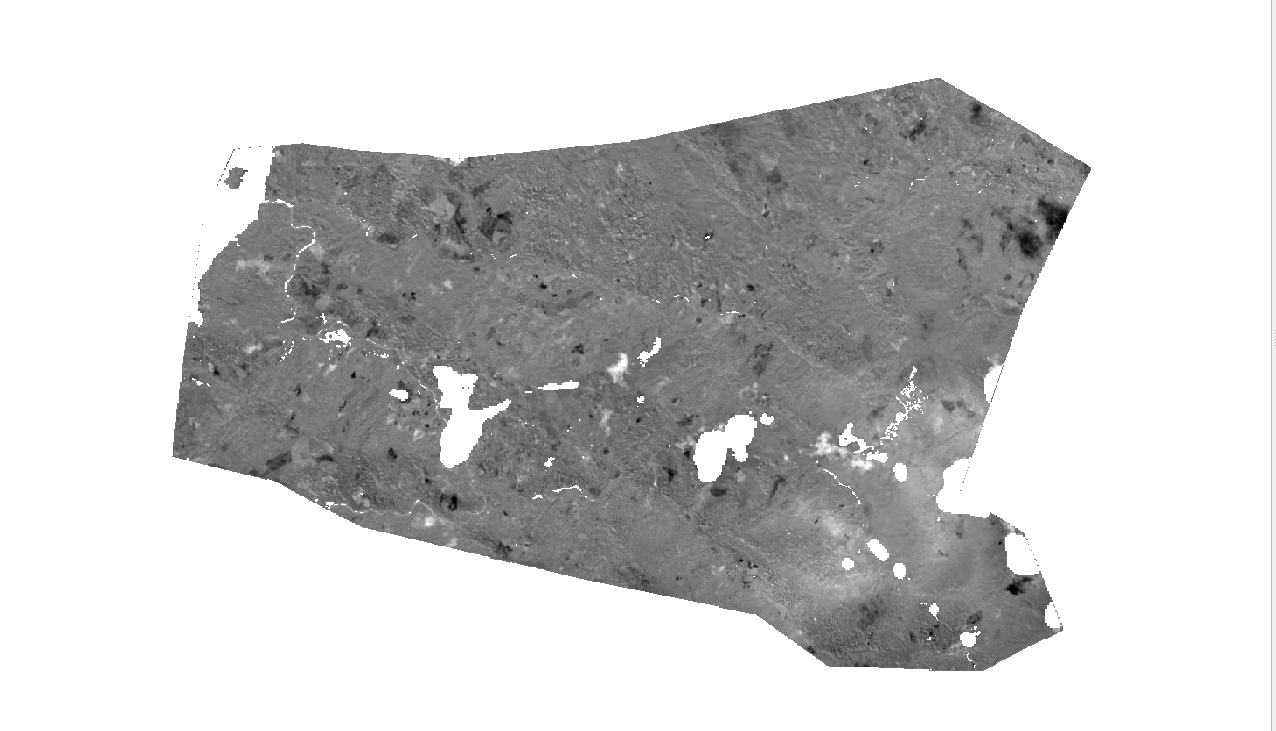
\includegraphics[width=\linewidth,height=0.6\textheight,keepaspectratio]{q_dnir.png}\\
{\small $\Delta NIR = B08_{t_2} - B08_{t_1}$}
\end{columns}
\end{frame}

% ---------------------------------------------------------------
\begin{frame}{Fase 4 -- Umbral, tamizado y vectorización}
\begin{columns}[T]
\column{0.5\textwidth}
\begin{itemize}
  \item $\mu = -0.00867$, $\sigma = 0.04195$ (471\,859 píxeles válidos).
  \item $T = \mu - 2\sigma = \mathbf{-0.0926}$
  \item Pérdida: $\Delta NDVI < T$ \textbf{y} $NDVI_{t_1} \ge 0.5$ (antes había vegetación).
  \item \textbf{Sieve} de 4 píxeles (400 m$^2$) para quitar ruido.
  \item \textbf{Polygonize} $\rightarrow$ capa \texttt{deslizamientos}, área con \texttt{area(\$geometry)/10000}.
\end{itemize}
\column{0.5\textwidth}\centering
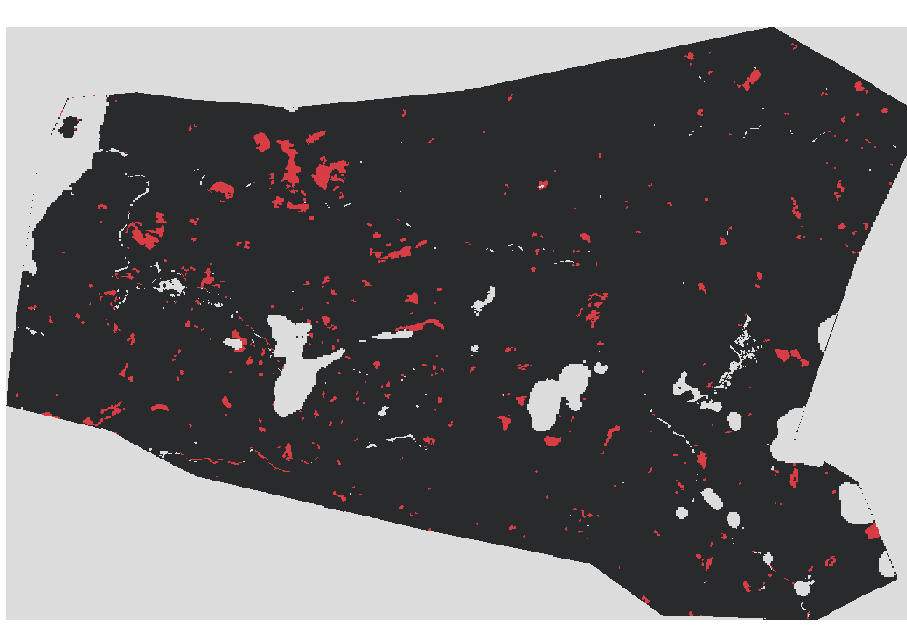
\includegraphics[width=\linewidth,height=0.72\textheight,keepaspectratio]{q_loss_sieve.png}\\{\small rojo = pérdida de vegetación}
\end{columns}
\end{frame}

% ---------------------------------------------------------------
\begin{frame}{Resultado: 374 deslizamientos, 117.48 ha}
\begin{columns}[T]
\column{0.55\textwidth}\centering
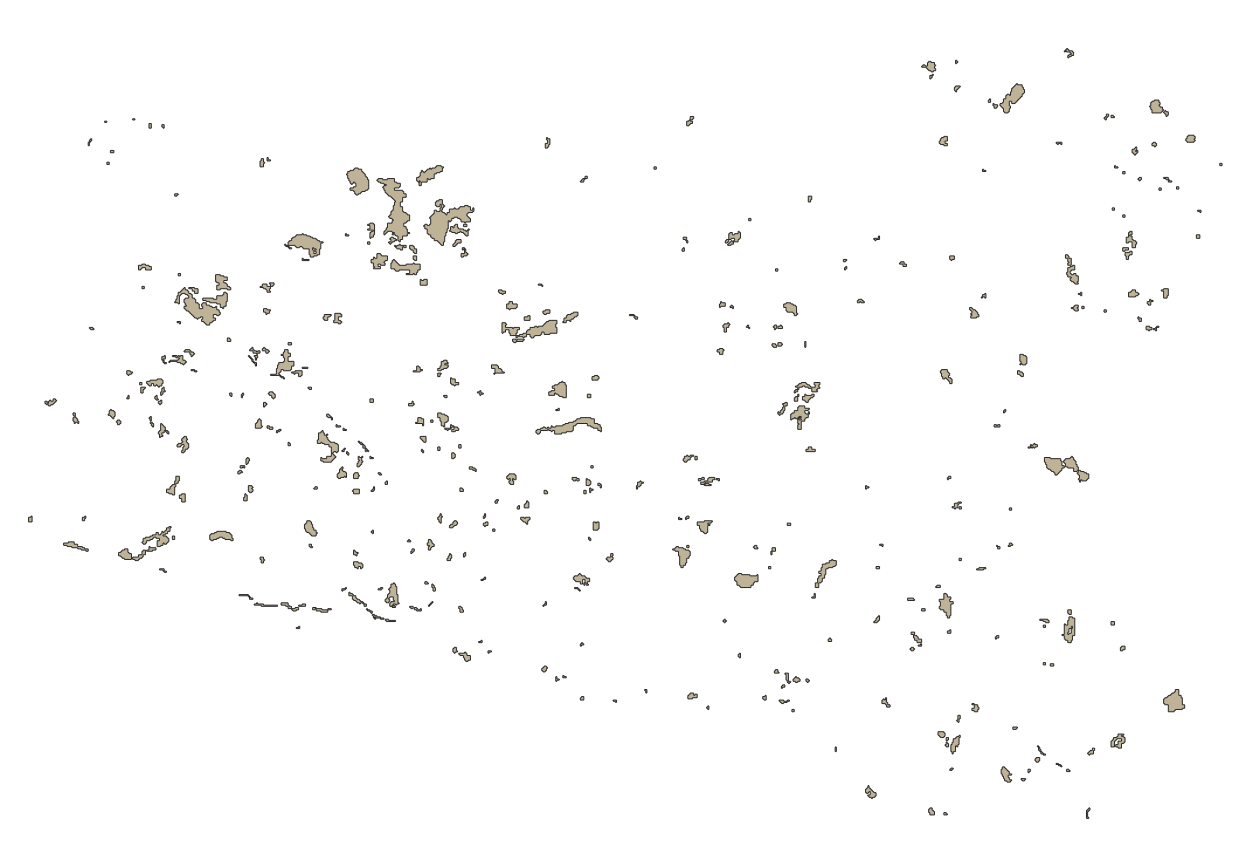
\includegraphics[width=\linewidth,height=0.72\textheight,keepaspectratio]{q_deslizamientos.png}
\column{0.45\textwidth}
\small
\begin{tabular}{lr}
\toprule
Polígonos & \textbf{374} \\
Área total & \textbf{117.48 ha} \\
\% del área válida & 2.5\% \\
Mayor / mediana & 6.27 / 0.11 ha \\
$<$0.5 ha & 320 \\
0.5--1 / 1--5 / $\ge$5 ha & 24 / 26 / 2 \\
\bottomrule
\end{tabular}

\vspace{3mm}
Conglomerado principal: \textbf{cañón alto del río Ingará}, al norte del río (noroeste).
\end{columns}
\end{frame}

% ---------------------------------------------------------------
\begin{frame}{Post-clasificación supervisada (SCP)}
\begin{columns}[T]
\column{0.36\textwidth}
\small
\begin{itemize}
  \item Un \textbf{band set} por fecha (6 bandas).
  \item 6 clases: bosque, pasto, \alert{suelo desnudo}, urbano, agua, nube/sombra.
  \item ROI de entrenamiento \textbf{por fecha}, con apoyo de Google Earth.
  \item \textbf{Random Forest}: 200 árboles, pesos balanceados.
\end{itemize}
\column{0.32\textwidth}\centering
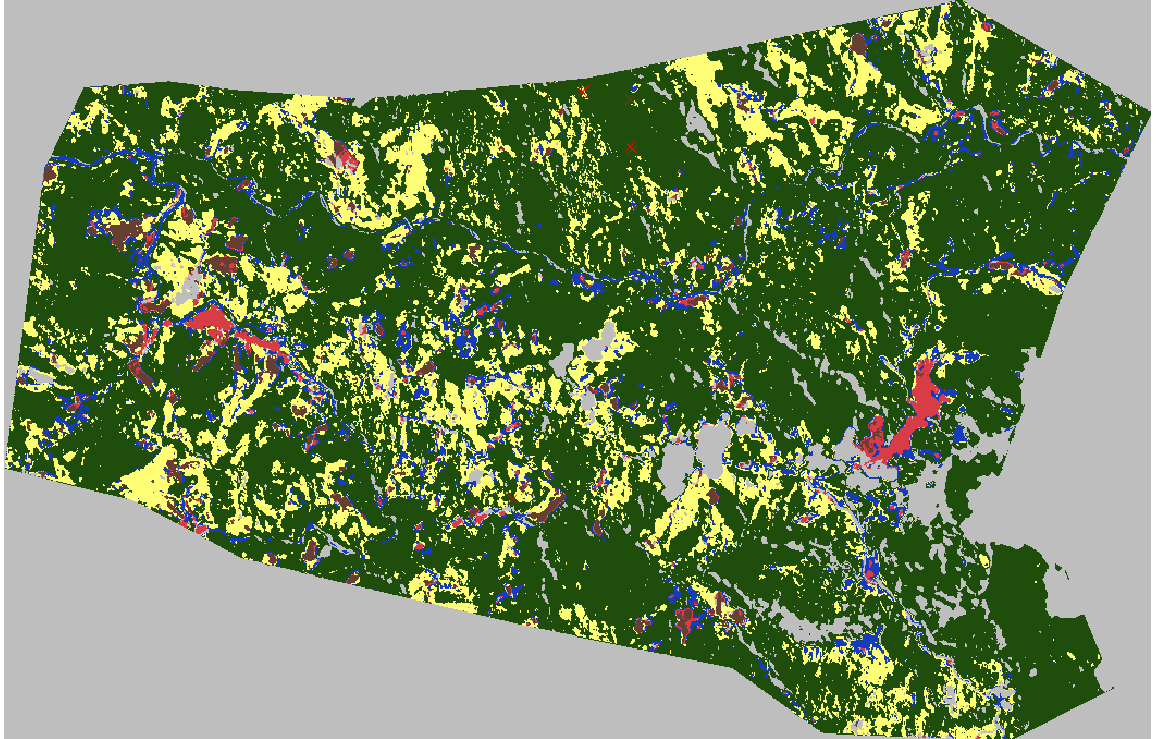
\includegraphics[width=\linewidth]{q_class_t1.png}\\{\small $t_1$}
\column{0.32\textwidth}\centering
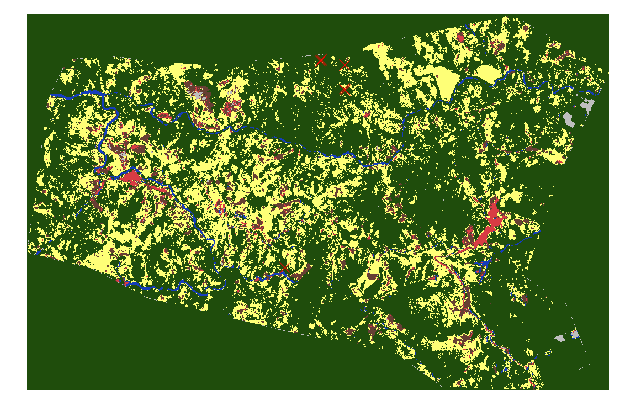
\includegraphics[width=\linewidth]{q_class_t2.png}\\{\small $t_2$}
\end{columns}
\end{frame}

% ---------------------------------------------------------------
\begin{frame}{Matriz de cambio \emph{De-A} (ha)}
\centering\small
\begin{tabular}{lrrrrrr}
\toprule
De $t_1$ \textbackslash{} A $t_2$ & Bosque & Pasto & Suelo & Urbano & Agua & Total $t_1$ \\
\midrule
Bosque & 2\,710.9 & 505.4 & \alert{\textbf{16.2}} & 2.4 & 16.0 & 3\,251.0 \\
Pasto  & 138.3 & 574.5 & \alert{\textbf{64.7}} & 16.8 & 4.0 & 798.3 \\
Suelo  & 3.6 & 36.3 & 46.6 & 6.1 & 0.0 & 92.5 \\
Urbano & 5.7 & 9.8 & 24.5 & 26.6 & 1.2 & 67.7 \\
Agua   & 79.2 & 93.7 & 37.2 & 1.6 & 32.4 & 244.1 \\
\midrule
Total $t_2$ & 2\,937.6 & 1\,219.7 & \textbf{189.1} & 53.5 & 53.5 & 4\,453.5 \\
\bottomrule
\end{tabular}

\vspace{3mm}
\begin{itemize}
  \item Suelo desnudo \textbf{se duplica}: 92.5 $\rightarrow$ 189.1 ha.
  \item Vegetación $\rightarrow$ suelo = \textbf{80.9 ha}, del mismo orden que el $\Delta$NDVI (117.5 ha).
  \item Bosque $\rightarrow$ pasto (505 ha) y agua $\rightarrow$ bosque/pasto: errores de clasificación, no cambios reales.
\end{itemize}
\end{frame}

% ---------------------------------------------------------------
\begin{frame}{Validación de las clasificaciones}
\begin{columns}[T]
\column{0.55\textwidth}
\small
\begin{tabular}{lrr}
\toprule
& $t_1$ & $t_2$ \\
\midrule
Exactitud global & 87.7\% & 91.2\% \\
\textbf{Kappa} & \textbf{0.811} & \textbf{0.825} \\
\textbf{F1 macro} & \textbf{0.822} & \textbf{0.883} \\
\midrule
F1 bosque & 0.923 & 0.944 \\
F1 pasto & 0.882 & 0.667 \\
F1 \alert{suelo/deslizamiento} & 0.644 & \alert{\textbf{0.805}} \\
F1 urbano & 0.973 & 0.983 \\
F1 agua & 0.678 & 0.981 \\
\bottomrule
\end{tabular}
\column{0.45\textwidth}
\small
\begin{itemize}
  \item Polígonos de validación \textbf{independientes} del entrenamiento.
  \item SCP \emph{Accuracy}; métricas recalculadas excluyendo los píxeles sin referencia.
  \item Kappa $>$ 0.80: casi perfecto (Landis y Koch).
  \item En $t_2$ el mapa encuentra el \textbf{91\%} del suelo desnudo real.
  \item Punto débil: confusión bosque--pasto.
\end{itemize}
\end{columns}
\end{frame}

% ---------------------------------------------------------------
\begin{frame}{Validación de los deslizamientos del $\Delta$NDVI}
\begin{columns}[T]
\column{0.5\textwidth}
\small
50 puntos aleatorios dentro y 50 fuera; cada uno revisado visualmente comparando $t_1$ y $t_2$.

\vspace{2mm}
\begin{tabular}{lrr}
\toprule
& Real: sí & Real: no \\
\midrule
$\Delta$NDVI: sí & TP = 39 & FP = 11 \\
$\Delta$NDVI: no & FN = 17 & TN = 33 \\
\bottomrule
\end{tabular}

\vspace{3mm}
\begin{tabular}{lr}
Exactitud global & 72\% \\
Precisión & \textbf{0.78} \\
Exhaustividad & 0.70 \\
\textbf{F1} & \textbf{0.74} \\
\textbf{Kappa} & \textbf{0.44} (moderado) \\
\end{tabular}
\column{0.5\textwidth}\centering
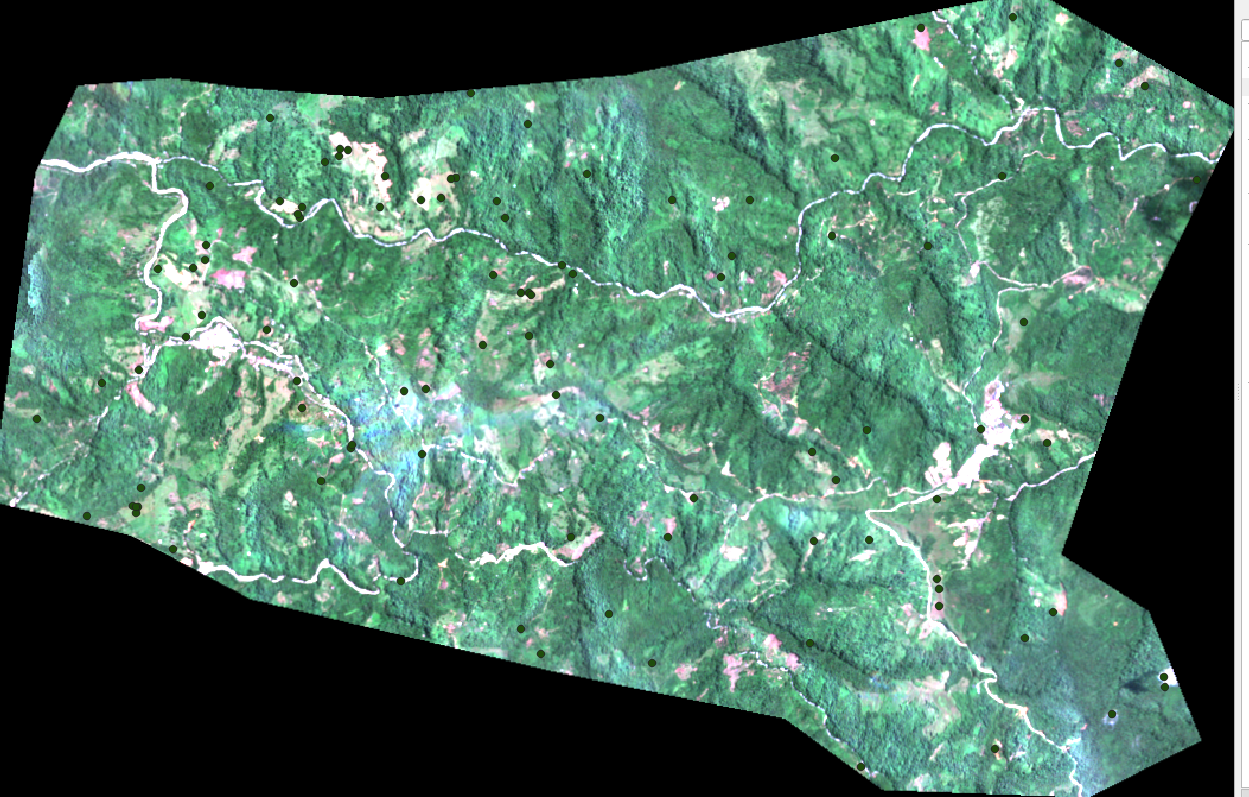
\includegraphics[width=\linewidth,height=0.55\textheight,keepaspectratio]{q_pts_etiquetado.png}

\small Método \textbf{conservador}: lo que detecta es confiable, pero omite $\sim$30\%.
\end{columns}
\end{frame}

% ---------------------------------------------------------------
\begin{frame}{Discusión}
\begin{itemize}
  \item La profundidad intermedia ($\sim$110 km) repartió la sacudida en un área amplia; las laderas empinadas, meteorizadas y saturadas fallaron.
  \item Los deslizamientos se concentran en el \textbf{cañón del Ingará} y en las vías: esto explica el \textbf{aislamiento} de San José del Palmar.
  \item Mucho del suelo nuevo viene de \textbf{pastos}: las laderas ganaderas son más vulnerables que el bosque.
  \item Los dos métodos se complementan: el $\Delta$NDVI \emph{dónde} y cuánto; la clasificación, \emph{de qué a qué}.
  \item Amenaza sísmica y amenaza por deslizamientos deben planearse juntas en el ordenamiento territorial.
\end{itemize}
\end{frame}

% ---------------------------------------------------------------
\begin{frame}{Limitaciones}
\begin{itemize}
  \item Nubosidad persistente: elección de fechas y 5.1\% del área enmascarada.
  \item El $\Delta$NDVI también capta cosechas o talas; no se aplicó un filtro de pendiente.
  \item A 10 m de resolución no se ven deslizamientos de menos de $\sim$0.04 ha, y los bordes de las cicatrices son píxeles mezclados.
  \item Sombras topográficas clasificadas como agua en $t_1$; confusión bosque--pasto en $t_2$.
  \item Validación visual sobre Sentinel-2 y Google Earth, sin imágenes de muy alta resolución posteriores al evento.
  \item Trabajo futuro: Sentinel-1 SAR para el daño urbano y para trabajar con nubes.
\end{itemize}
\end{frame}

% ---------------------------------------------------------------
\begin{frame}{Conclusiones}
\begin{itemize}
  \item Flujo reproducible con datos gratuitos (Sentinel-2 L2A) y software libre (QGIS + SCP).
  \item \textbf{374 deslizamientos, 117.48 ha} (2.5\% del área válida), concentrados en el cañón del río Ingará.
  \item La post-clasificación confirma el daño: el suelo desnudo se duplica y 80.9 ha de vegetación pasan a suelo.
  \item Exactitud: clasificaciones con Kappa $>$ 0.80; deslizamientos $\Delta$NDVI con F1 = 0.74.
  \item Una herramienta rápida para apoyar la atención de la emergencia en zonas montañosas, nubladas y de difícil acceso.
\end{itemize}
\end{frame}

\begin{frame}[standout]
¡Gracias!\\[3mm]
\normalsize ¿Preguntas?
\end{frame}

\end{document}
